%%%%%%%%%%%%%%%%%%%%%%%%%%%%%%%%%%%%%%%%%%%%
% FILE INI JANGAN DI UBAH
%%%%%%%%%%%%%%%%%%%%%%%%%%%%%%%%%%%%%%%%%%%%
%\usepackage[indonesian]{babel}
\usepackage[american]{babel}
%\usepackage[indonesian]{babel}
\usepackage[table,xcdraw]{xcolor}


\usepackage[pdfauthor={Nur Afandi},bookmarksnumbered,pdfborder={0 0 0}]{hyperref}
\usepackage[ruled,lined,commentsnumbered,linesnumbered]{algorithm2e}
\usepackage[utf8]{inputenc}
\usepackage{graphicx}
\usepackage{lipsum}
\usepackage{hyphenat}
\usepackage{rotating}
\usepackage{booktabs}
\usepackage{lscape}
%\usepackage{algpseudocode}
\usepackage[ruled,lined,commentsnumbered,linesnumbered]{algorithm2e}
\usepackage{algpseudocode}
\usepackage{makeidx}
\usepackage{rotating}
\makeindex
\usepackage{epsfig}
\usepackage{subfig}
\usepackage{pdflscape}
\usepackage[doublespacing]{setspace}
\setstretch{1.5}
\usepackage{type1cm}
\usepackage{longtable}
\usepackage{lscape}
\usepackage{lettrine}
\usepackage{hyperref}
\usepackage[pageref]{backref}
\usepackage{multirow}
\usepackage[table,xcdraw]{xcolor}
\usepackage{eso-pic}
\newcommand\BackgroundIm{
	\put(0,0){
		\parbox[b][\paperheight]{\paperwidth}{%
			\vfill
			\centering
			\includegraphics[height=\paperheight,
				keepaspectratio]{./lib/background.png}%
			\vfill
		}}}

\usepackage{fancyhdr} % Untuk pengaturan header dan footer yang lebih kompleks
\usepackage{etoolbox} % Untuk melakukan perubahan (patch) command internal LaTeX
\usepackage{url}
\usepackage{longtable}
\usepackage{float}
\usepackage{morefloats}
\floatstyle{boxed}
\newfloat{program}{thp}{lop}
\floatname{program}{Program}
\usepackage[fleqn]{amsmath}
\usepackage{nccmath}
\usepackage{enumitem}
\usepackage{ulem}
\usepackage[final]{pdfpages}
\usepackage{titlesec}
\usepackage{array}
\usepackage{multicol}
\usepackage{listings}
\usepackage{wrapfig}
\usepackage{array,tabularx}
\usepackage{lscape}
\usepackage{longtable}
\usepackage{caption}
\usepackage[export]{adjustbox}
\usepackage{ragged2e}
\usepackage{epsfig}
\usepackage{subfig}
\usepackage[top=35mm,left=40mm,right=30mm,bottom=30mm]{geometry}
\usepackage{pdflscape}
\usepackage[doublespacing]{setspace}
\setstretch{1.5}
\usepackage{type1cm}
\usepackage{lettrine}
\usepackage{hyperref}
\usepackage[pageref]{backref}
\usepackage{multirow}
\usepackage[table,xcdraw]{xcolor}
\usepackage{fancyhdr} % Untuk pengaturan header dan footer yang lebih kompleks
\usepackage{etoolbox} % Untuk melakukan perubahan (patch) command internal LaTeX
\usepackage{url}
\usepackage{longtable}
\usepackage{float}
\usepackage{morefloats}
\floatstyle{boxed}
\newfloat{program}{thp}{lop}
\floatname{program}{Program}
\usepackage[fleqn]{amsmath}
\usepackage{enumitem}
\usepackage{ulem}
\usepackage[final]{pdfpages}
\usepackage{titlesec}
\usepackage{array}
\usepackage{multicol}
\usepackage{listings}
\usepackage{wrapfig}
\usepackage{array,tabularx}
\usepackage{longtable}
\usepackage{caption}
%\usepackage{natbib}
%\usepackage[numbers]{natbib}
\usepackage[numbers]{natbib}
\usepackage{siunitx}
\usepackage{dirtree}
\usepackage{hyperref}
\usepackage{adjustbox}

%\usepackage[sorting=none]{biblatex}

%square,sort,comma,numbers

%\renewcommand{\uline}[1]{\textit{#1}}
%\bibliographystyle{apalike}
\usepackage[export]{adjustbox}
\usepackage{ragged2e}
\usepackage[utf8]{inputenc}
\usepackage{afterpage}
\usepackage{lipsum}
%\usepackage{cite}
% More tidy url
%\usepackage{url}
%\usepackage{breakurl}
%\def\UrlBreaks{\do\/\do-\do.}

% Set paper size and margin
\usepackage{geometry}
\geometry{
	a4paper,
	left=40mm,
	top=35mm,
	right=30mm,
	bottom=30mm,
}

% untuk Cover
\newenvironment{FontCover}{\fontfamily{phv}\selectfont}{\par}
% untuk Lembar Pengesahan
\newenvironment{Kondisi}
{\par\vspace{\abovedisplayskip}\noindent
\tabularx{\columnwidth}{>{$}l<{$} @{${}:{}$} >{\raggedright\arraybackslash}X}}
	{\endtabularx\par\vspace{\belowdisplayskip}}
	\newenvironment{Kondisi2}
	{\par\vspace{\abovedisplayskip}\noindent
	\tabularx{\columnwidth}{>{$}l<{$} @{${}:{}$} >{\raggedright\arraybackslash}X}}
{\endtabularx\par\vspace{\belowdisplayskip}}
% Line spacing
\linespread{1.5}

% fix titlesec bug
\makeatletter
\patchcmd{\ttlh@hang}{\parindent\z@}{\parindent\z@\leavevmode}{}{}
\patchcmd{\ttlh@hang}{\noindent}{}{}{}
\makeatother

% Pengaturan format Chapter dan Section
\titleformat{\chapter}[display]{\bfseries\Large}{BAB \centering\thechapter}{0ex}{\vspace{0ex}\centering}[\vspace{3ex}]
\titlespacing*{\chapter}{0pt}{-4ex}{0pt}
\titleformat{\section}{\bfseries\normalsize}{\MakeUppercase{\thesection}}{1ex}{}
\titleformat{\subsection}{\normalsize\bfseries}
\titleformat{\subsubsection}{\normalsize\bfseries}

\titlespacing{\section}{0pt}{0pt}{1ex}
\titlespacing{\subsection}{0pt}{0pt}{1ex}
\titlespacing{\subsubsection}{0pt}{0pt}{1ex}

% Keterangan rumus
\newenvironment{conditions}
{\par\vspace{\abovedisplayskip}\noindent
\tabularx{\columnwidth}{>{$}l<{$} @{${}={}$} >{\raggedright\arraybackslash}X}}
{\endtabularx\par\vspace{\belowdisplayskip}}

% Caption label bold
\usepackage[labelfont=bf]{caption}
\captionsetup{labelfont=bf}

% Jarak caption dengan obyek
\captionsetup[figure]{font=small,skip=15pt}
\captionsetup[table]{font=small,skip=15pt}


\DeclareCaptionLabelSeparator{none}{}
\captionsetup{labelsep=period}
% Caption nama
\renewcommand{\figurename}{Gambar}
\renewcommand{\tablename}{Tabel}
\renewcommand{\lstlistingname}{Kode}

% Cek nomor halaman
\usepackage{changepage}

% Cek spelling
\usepackage{lipsum}
\setcounter{secnumdepth}{5}
\hyphenation{meng-gerak-kan mem-per-kenal-kan pe-ri-la-ku di-je-las-kan mem-bu-tuh-kan me-ne-rap-kan}

% Definisi untuk "halaman sengaja dikosongkan"
\def\kosong{
	\vspace*{\fill}
	\begin{center}\textit{This page is intentionally left blank}\end{center}
	\vfill
}

% Halaman sengaja dikosongkan
\patchcmd{\cleardoublepage}{\hbox{}}{\kosong}{}{}
% Untuk citation
%\newcommand{\tab}[1]{\hspace{.2\textwidth}\rlap{#1}}
\renewcommand*{\backreflastsep}{, }
\renewcommand*{\backreftwosep}{, }
\renewcommand*{\backref}[1]{}
%\renewcommand*{\backrefalt}[4]{
%	\ifcase #1
%	No citations.
%	\or
%	(Dikutip pada halaman #2).
%	\else
%	(Dikutip pada halaman #2).
%	\fi
%}
% Pengaturan penomoran halaman menggunakan package fancyhdr
\fancyhf{} 								% Mengosongkan header dan footer
\renewcommand{\headrulewidth}{0pt} 		% Menghapus garis horizontal pada header
\pagestyle{fancy} 						% Mengubah pagestyle dokumen menjadi fancy
\fancyfoot[CE,CO]{\thepage}				% Footer kanan pada hal. ganjil dan sebaliknya
%\patchcmd{\chapter}{plain}{fancy}{}{} 	% Mengubah pagestyle pada chapter menjadi fancy
\patchcmd{\chapter}{empty}{plain}{}{}
\usepackage{ifthen}
\newboolean{PembimbingDua}
\setboolean{PembimbingDua}{false}
\newboolean{bThesis}
\setboolean{bThesis}{true}

%\newcommand{\Tesis}
%{	\setboolean{bThesis}{true}
%}



\newboolean{PembimbingTiga}
\setboolean{PembimbingTiga}{false}

\newboolean{PengujiTiga}
\setboolean{PengujiTiga}{false}

\newboolean{PengujiEmpat}
\setboolean{PengujiEmpat}{false}

\newboolean{Nomenklatur}
\setboolean{Nomenklatur}{false}

\newboolean{bDoktor}
\setboolean{bDoktor}{false}
\newboolean{bMaster}
\setboolean{bMaster}{false}

\renewcommand{\em}[1]{\textit{#1}}
\renewcommand{\emph}[1]{\textit{#1}}

\newcommand{\Mahasiswa}[2]{
	\newcommand{\NamaMahasiswa}{#1}
	\newcommand{\NrpMahasiswa}{#2}
}
\newcommand{\PembimbingSatu}[2]
{
	\newcommand{\PbSatu}{#1}
	\newcommand{\NipPbSatu}{#2}
}
\newcommand{\PembimbingDua}[2]{
	\setboolean{PembimbingDua}{true}
	\newcommand{\PbDua}{#1}
	\newcommand{\NipPbDua}{#2}
}

\newcommand{\PembimbingTiga}[2]{
	\setboolean{PembimbingTiga}{true}
	\newcommand{\PbTiga}{#1}
	\newcommand{\NipPbTiga}{#2}
}

\newcommand{\PengujiSatu}[2]
{
	\newcommand{\PjSatu}{#1}
	\newcommand{\NipPjSatu}{#2}
}
\newcommand{\PengujiDua}[2]
{	\newcommand{\PjDua}{#1}
	\newcommand{\NipPjDua}{#2}
}
\newcommand{\PengujiTiga}[2]
{
	\setboolean{PengujiTiga}{true}
	\newcommand{\PjTiga}{#1}
	\newcommand{\NipPjTiga}{#2}
}

\newcommand{\PengujiEmpat}[2]
{
	\setboolean{PengujiEmpat}{true}
	\newcommand{\PjEmpat}{#1}
	\newcommand{\NipPjEmpat}{#2}
}
\newcommand{\KaDep}[2]
{
	\newcommand{\NmKaDep}{#1}
	\newcommand{\NipKaDep}{#2}
}
\newcommand{\CoverFooter}[1]
{\newcommand{\bdk}{#1}
}
\newcommand{\Judul}[1]
{
	\newcommand{\JdTesis}{#1}
}
\newcommand{\TanggalUjian}[1]
{
	\newcommand{\TglUjian}{#1}
}
\newcommand{\PeriodeWisuda}[1]
{
	\newcommand{\PerWisuda}{#1}
}

\newcommand{\Fakultas}[1]
{
	\newcommand{\fak}{#1}
}
\newcommand{\BeltFakultas}[1]
{
	\newcommand{\bbelt}{#1}
}
\newcommand{\Departemen}[1]
{
	\newcommand{\Dep}{#1}
}
\newcommand{\ggGelar}{xxxx}
\newcommand{\pPengesahan}{xxxxxxxx}

\newcommand{\Gelar}[1]
{
	\renewcommand{\ggGelar}{#1}
}

\newcommand{\tsss}{Disertasi disusun untuk memenuhi salah satu syarat memperoleh gelar}

\newcommand{\Disertasi}[1]
{\renewcommand{\tsss}{Disertasi disusun untuk memenuhi salah satu syarat memperoleh gelar}
	\renewcommand{\pPengesahan}{LEMBAR PENGESAHAN DISERTASI}
	\renewcommand{\ggGelar}{#1}
	\setboolean{bMaster}{false}
	\setboolean{bThesis}{true}
}

\newcommand{\prop}{PROPOSAL DISERTASI}
\newcommand{\ProposalDisertasi}
{	\renewcommand{\prop}{PROPOSAL DISERTASI}
	\setboolean{bMaster}{false}
	\setboolean{bThesis}{false}
}

\newcommand{\Tesis}[1]
{
	\renewcommand{\tsss}{The thesis is written to fulfill one of the requirements for obtaining a degree
		of}
	\renewcommand{\pPengesahan}{THESIS VALIDATION SHEET}
	\setboolean{bMaster}{true}
	\setboolean{bThesis}{true}
	\renewcommand{\ggGelar}{#1}

}

\newcommand{\ProposalTesis}
{	\setboolean{bMaster}{true}
	\renewcommand{\prop}{THESIS PROPOSAL}
	\setboolean{bThesis}{false}
}


\newboolean{JudulTesisEng}
\setboolean{JudulTesisEng}{true}

\newcommand{\JudulEng}[1]
{
	\setboolean{JudulTesisEng}{true}
	\newcommand{\JdTesisEng}{#1}
}

\newcommand{\Kode}[1]
{\newcommand{\Kodekk}{#1}
}

\newcommand{\TempatUjian}[1]
{
	\newcommand{\bTempatUjian}{#1}
}

\newcommand{\HariUjian}[1]
{
	\newcommand{\bHariUjian}{#1}
}

\newcommand{\DaftarRiwayatHidup}{
\addcontentsline{toc}{chapter}{Author Biography}
\titlespacing*{\chapter}{0pt}{0ex}{5ex}
\appendix
\chapter*{AUTHOR BIOGRAPHY}
%*********************************
%Gambar Foto 
\begin{center}
	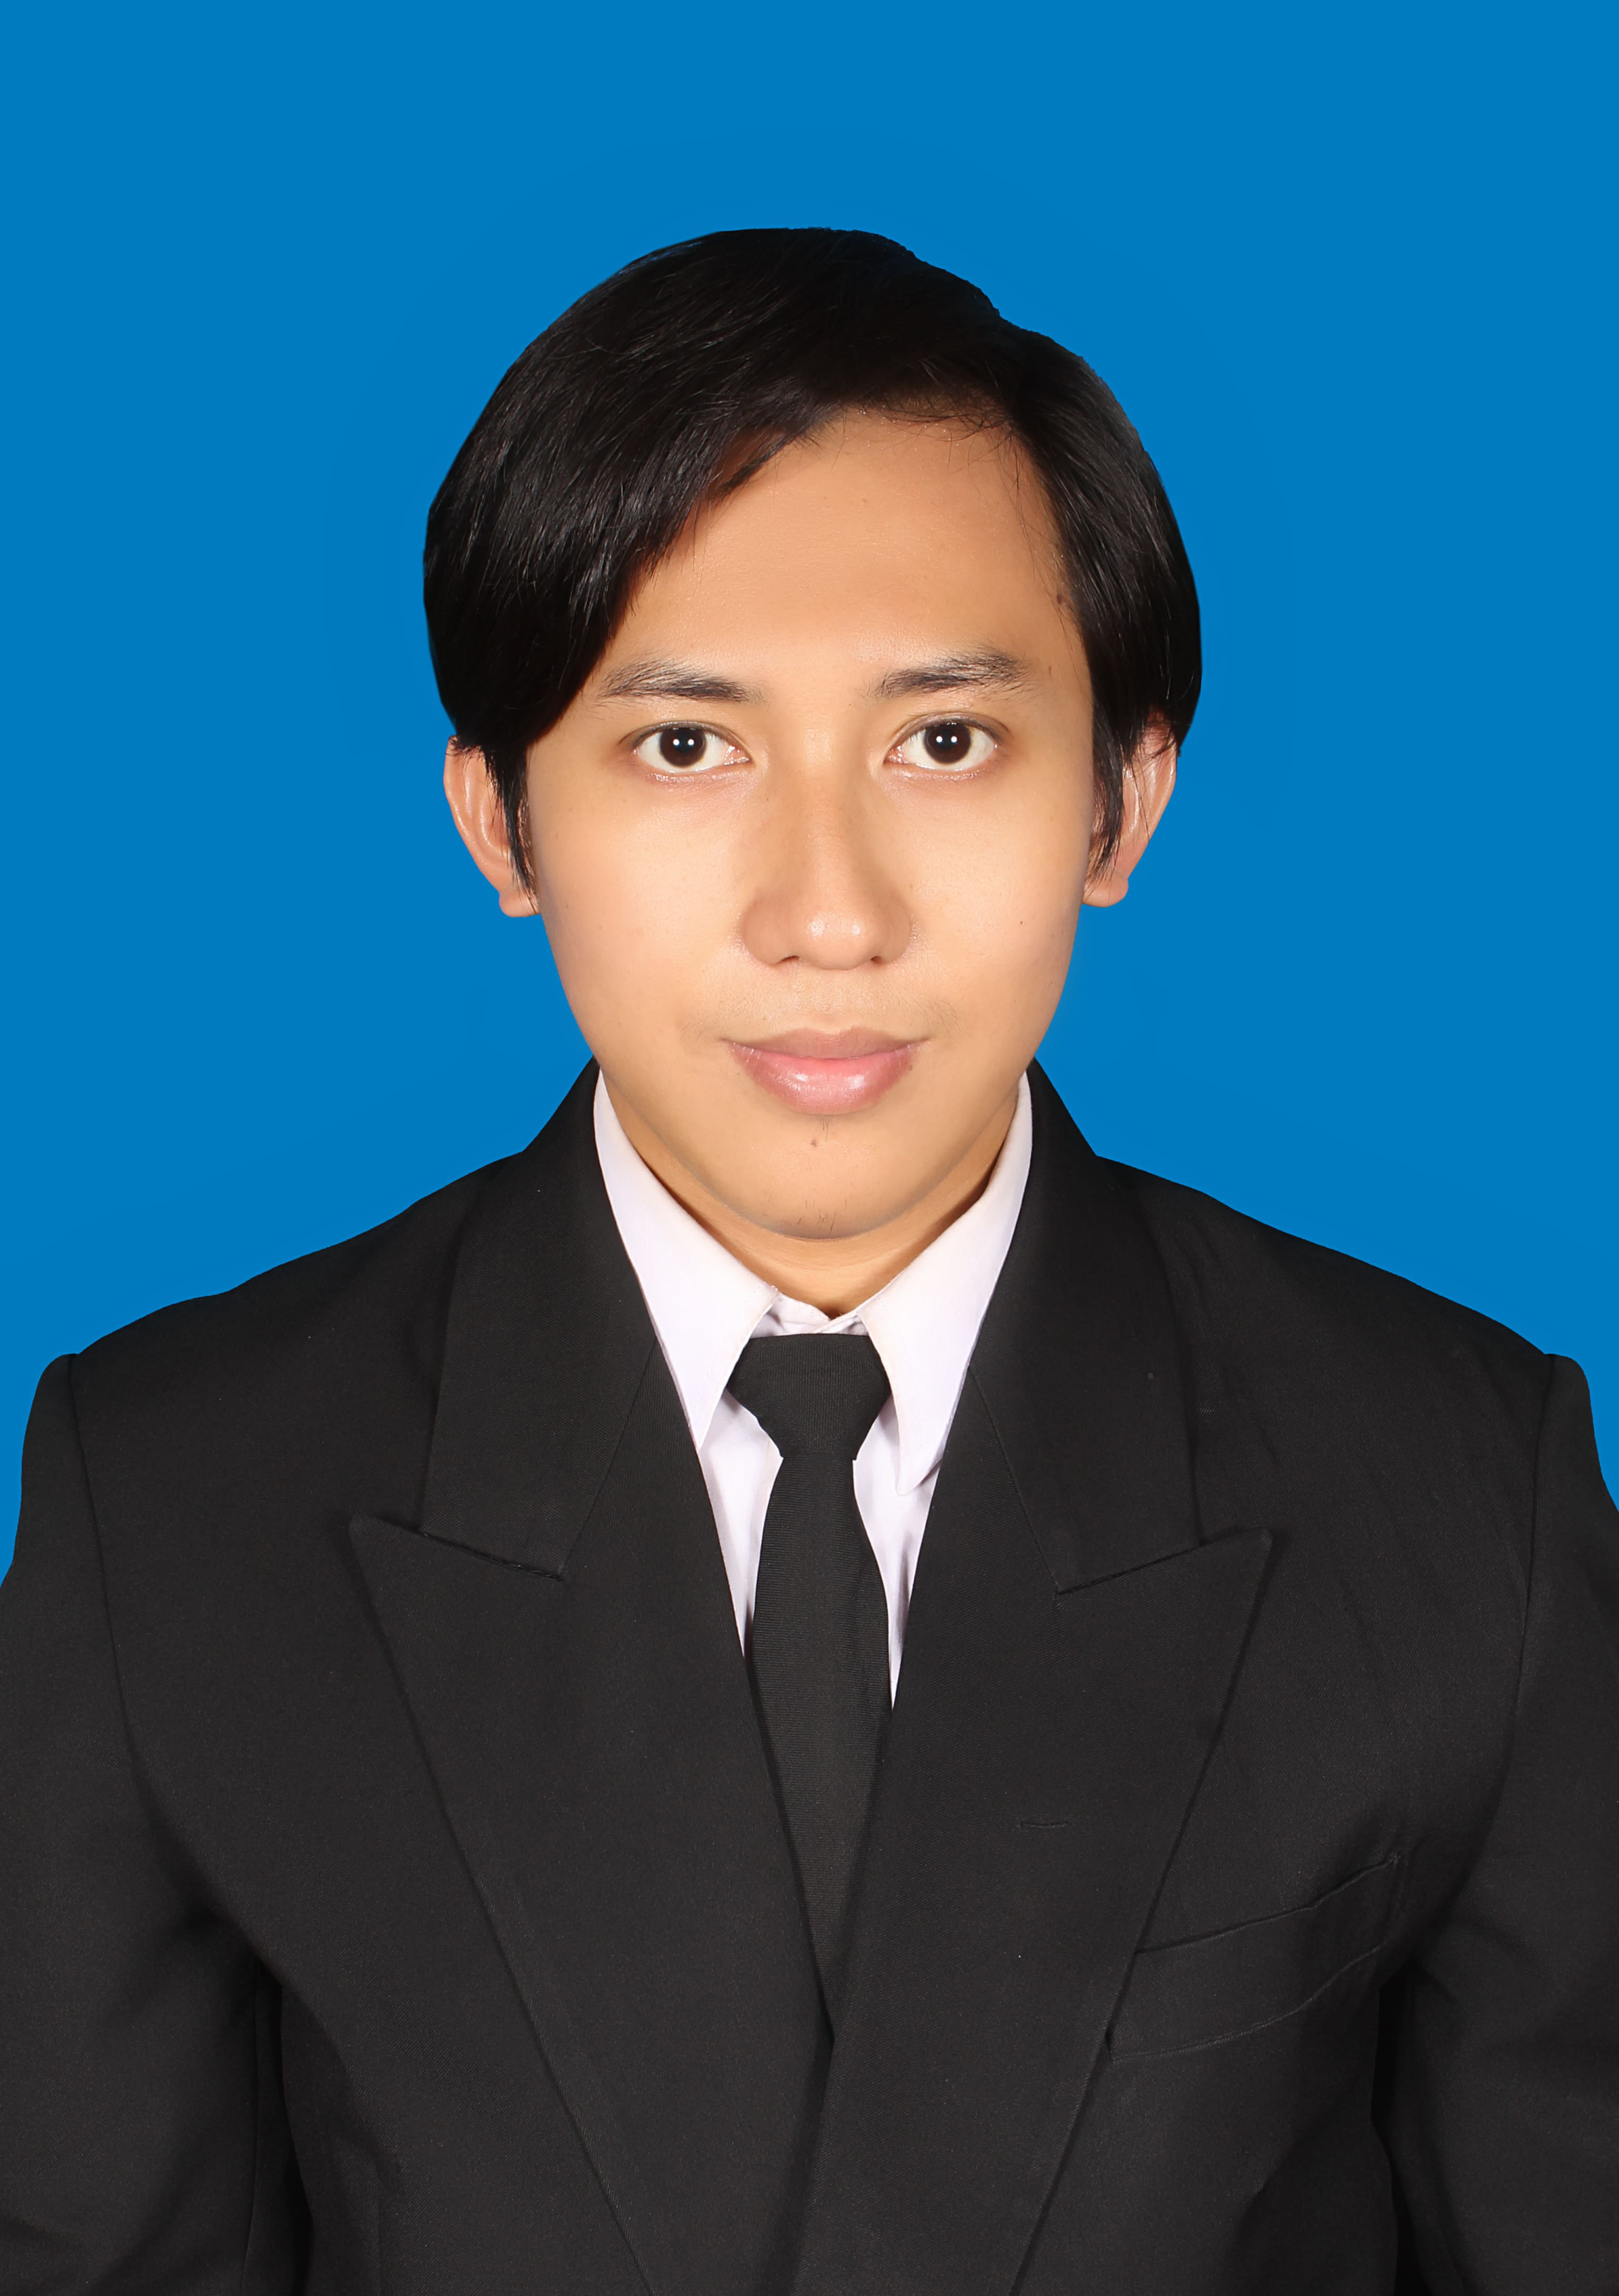
\includegraphics[height=0.2\textheight]{./ubah/foto_amik.jpg}
\end{center}
%*********************************
\section*{Personal Identity}
\begin{tabular}{p{3cm}cp{9cm}}
	%Masukan Identitas Disini.............
	Nama          & : &
	Amik Rafly Azmi Ulya                           \\
	Tempat Lahir  & : &
	Jepara                                         \\
	Tanggal Lahir & : &
	14 November 1999                               \\
	Alamat        & : &
	Mangkuyudan, Kartasura, Sukoharjo, Jawa Tengah \\
\end{tabular}

\section*{Educational Background}
\begin{tabular}{p{3cm}cp{9cm}}
	2022-2024 & : &
	Master Degree (S2), Department of Electrical Engineering, Faculty of Intelligent Electrical and Informatics Technology, Institut Teknologi Sepuluh Nopember \\
	          &   &                                                                                                                                             \\
	2018-2022 & : &
	Bachelor Degree (S1), Departement of Physics, Faculty of Science and Data Analytics, Institut Teknologi Sepuluh Nopember                                    \\
	          &   &                                                                                                                                             \\
	2015-2018 & : &
	2\textsuperscript{nd} Kudus Islamic State Senior High School (MAN)                                                                                          \\
	          &   &                                                                                                                                             \\
	2012-2015 & : &
	Unggulan Pondok Modern Selamat Junior High School (SMP)                                                                                                     \\
	          &   &                                                                                                                                             \\
	2006-2012 & : &
	Al-Islam Kartasura Islamic Elementary School (MI)                                                                                                           \\
\end{tabular}


\section*{Publication List}

\begin{enumerate}
	\item Amik Rafly Azmi Ulya et al. “HiroPoseEstimation: A Dataset of Pose Estimation for Kid-Size Humanoid Robot”. In: Journal of Information Technology and Computer Science 8.3 (2023), 231–240. DOI: 10.25126/ jitecs.202383568. URL: https://jitecs.ub.ac.id/index.php/ jitecs/article/view/568.
\end{enumerate}

% \section*{Riwayat Penelitian}
% \begin{enumerate}
% 	\item \lipsum[3]
% 	\item \lipsum[3]
% 	\item Penelitian Ke Tiga
% 	\item Penelitian Ke Empat
% \end{enumerate}
% \section*{Riwayat Lainnya}

% \lipsum[1]
\cleardoublepage}


\newcommand{\DaftarPustaka}{%\\renewcommand\bibname{Daftar Pustaka}
%\\addcontentsline{toc}{chapter}{\bibname}
%\\titlespacing*{\chapter}{0pt}{0ex}{5ex}
%\\appendix
%\%\bibliographystyle{apalike}
%\%\bibliographystyle{ieetr}
%\%\bibliographystyle{IEEEtranN}
%\\bibliographystyle{plainnat}
%\\bibliography{./ubah/pustaka}
%\\cleardoublepage
%\gdef \bibname{Daftar Pustaka}
\renewcommand \bibname {Bibliography}
\addcontentsline{toc}{chapter}{\bibname}
\titlespacing*{\chapter}{0pt}{0ex}{5ex}
\appendix
%\bibliographystyle{IEEEtranN}
\bibliographystyle{IEEEtran}
\bibliography{IEEEabrv,./ubah/pustaka.bib}
%\bibliography{IEEEabrv,pustaka.bib}
%\bibliography{../ubah/pustaka.bib}
%\bibliography{library}
\cleardoublepage}

\tolerance=9999
\emergencystretch=10pt
\hyphenpenalty=10000
\exhyphenpenalty=100